\def\year{2019}\relax
%File: formatting-instruction.tex
\documentclass[letterpaper]{article} %DO NOT CHANGE THIS
%\usepackage{aaai19}  %Required
\usepackage{times}  %Required
\usepackage{helvet}  %Required
\usepackage{courier}  %Required
\usepackage{url}  %Required
\usepackage{graphicx}  %Required
\frenchspacing  %Required
\setlength{\pdfpagewidth}{8.5in}  %Required
\setlength{\pdfpageheight}{11in}  %Required

%% Added the following
\usepackage[utf8]{inputenc} % allow utf-8 input
%\usepackage[T1]{fontenc}    % use 8-bit T1 fonts
\usepackage{hyperref}       % hyperlinks
%\usepackage{url}            % simple URL typesetting
\usepackage{booktabs}       % professional-quality tables
\usepackage{amsfonts}       % blackboard math symbols
\usepackage{nicefrac}       % compact symbols for 1/2, etc.
\usepackage{microtype}      % microtypography
\usepackage{xcolor}
\usepackage{bm}
\usepackage{xr}

\usepackage[accepted]{icml2019}

\newenvironment{thma}[1]{\par\noindent{\bf Theorem #1\ }\em}{\em}

\usepackage{array,multirow,graphicx}
\usepackage{float}

\externaldocument{ms}

\newtheorem{thm}{Theorem}

\usepackage{natbib}
\usepackage{tikz}
\usepackage{epsfig,amssymb,amsmath,ifthen,comment}
\newcommand{\red}{\textcolor{red}}
\newcommand{\E}{\mathbb{E}}
\DeclareMathOperator{\pa}{pa}
\DeclareMathOperator{\ch}{ch}

\DeclareMathOperator*{\argmax}{arg\,max}
\DeclareMathOperator*{\argmin}{arg\,min}

\newenvironment{prf}{\noindent\textit{Proof:}\begin{mdseries}}{\end{mdseries}{\hfill\scriptsize$\Box$}} 

%%

%PDF Info Is Required:
  \pdfinfo{
/Title (Supplemental Appendix)
/Author (Authors)}
\setcounter{secnumdepth}{0}  
 \begin{document}
% The file aaai.sty is the style file for AAAI Press 
% proceedings, working notes, and technical reports.
%
%\title{Supplemental Appendix for ``Learning Optimal Fair Policies''}
%\author{Razieh Nabi \\
%Affiliation\\
%}

\twocolumn[
%\icmltitle{{\color{blue}Breaking the Cycle Of Injustice Via Learning Fair Policies}}
\icmltitle{Supplemental Appendix for ``Learning Optimal Fair Policies''}

% It is OKAY to include author information, even for blind
% submissions: the style file will automatically remove it for you
% unless you've provided the [accepted] option to the icml2019
% package.

% List of affiliations: The first argument should be a (short)
% identifier you will use later to specify author affiliations
% Academic affiliations should list Department, University, City, Region, Country
% Industry affiliations should list Company, City, Region, Country

% You can specify symbols, otherwise they are numbered in order.
% Ideally, you should not use this facility. Affiliations will be numbered
% in order of appearance and this is the preferred way.
\icmlsetsymbol{equal}{*}

\begin{icmlauthorlist}
	%\icmlauthor{Aeiau Zzzz}{equal,to}
	\icmlauthor{Razieh Nabi}{to}
	\icmlauthor{Daniel Malinsky}{to}
	\icmlauthor{Ilya Shpitser}{to}
\end{icmlauthorlist}

%\icmlaffiliation{to}{Department of Computation, University of Torontoland, Torontoland, Canada}
\icmlaffiliation{to}{Department of Computer Science, Johns Hopkins University, Baltimore, MD, USA}

%\icmlcorrespondingauthor{Cieua Vvvvv}{c.vvvvv@googol.com}
\icmlcorrespondingauthor{Razieh Nabi}{rnabi@jhu.edu}

% You may provide any keywords that you
% find helpful for describing your paper; these are used to populate
% the "keywords" metadata in the PDF but will not be shown in the document
\icmlkeywords{Fair Policies, Policy Learning, Causal Inference, Mediation Analysis, Algorithmic Fairness}

\vskip 0.3in
]

\printAffiliationsAndNotice{}  % leave blank if no need to mention equal contribution
%\printAffiliationsAndNotice{\icmlEqualContribution} % otherwise use the standard text.



\section*{Appendix A: G-estimation}
G-estimation applies to structural nested models, which directly model the counterfactual deviations in outcome from a reference treatment value (which we take to be $A=0$) conditional on history, assuming all future decisions are already optimal. Specifically, for each decision point $k$ we posit a \emph{structural nested mean
	model (SNMM)} parameterized by $\psi$ as follows: %$\gamma_i(H_i, A_i; \psi)$ for the contrast
{\small
\begin{align*}
\gamma_k(H_k, &a_k; \psi) =\\
&\E[ Y(\bar{a}_{k-1}, a_k, f^*_{\underline{A}_{k+1}}) - Y(\bar{a}_{k-1}, a_k=0, f^*_{\underline{A}_{k+1}}) \mid H_k ],  
\end{align*}
}%
where $\underline{A}_{k+1}$ represents all treatments administered from time $k+1$ onwards. In words, $\gamma_k$ is the contrast of the counterfactual mean (conditional on observed history $H_k$) where the past decisions are set to their observed values, the present decision is either $a_k$ or a reference decision $a_k = 0$, and all future decisions are made optimally, $f^*_{\underline{A}_{k+1}}$.  

Note that if the true $\gamma_k(H_k,a_k;\psi)$ were known, the optimal treatment policies are those that maximize this ``blip'' function at each stage: $f^*_{A_k} = \argmax_{a_k} \gamma_k(H_k, a_k; \psi)$.
In order to estimate $\psi$ using data, let 
{\small
	\begin{align}
	U({\bf \psi, \zeta(\psi), \alpha}) = \sum_{k=1}^{K} &\left\{ G_k({\bf \psi}) - \E\left[G_k({\bf \psi}) \mid H_k; % , A_i;
	{\bf \zeta} \right] \right\} 
	\nonumber \\
	\times \ &\left\{ d_k(H_k, A_k) - E\left[d_k(H_k, A_k) \mid H_k; {\bf \alpha}\right] \right\}, 
	\label{eqn:G-estim}
	\end{align}
}%
where $d_k(H_k, A_k)$ is any function of $H_k$ and $A_k$ and $G_k({\bf \psi})$ is defined as 
{\small
	\begin{align*}
	Y  - \gamma_k(H_k, a_k; {\bf \psi}) + \sum_{i = k + 1}^{K} \left[ \gamma_i(H_i, a^*_i; {\bf \psi}) - \gamma_i(H_i, a_i; {\bf \psi}) \right],
	\end{align*}
}%
($a^*_i$ is the optimal decision at $i$th stage).   
Consistent estimators of ${\bf \psi}$ can be obtained solving the estimating equations $\E[U({\bf \psi, \zeta(\psi), \alpha})] = 0$, as shown in \citet{robins04SNMM}. 

Both of the modifications discussed for Q-learning and value search must be applied when learning fair optimal policies by g-estimation.  Specifically, we determine optimal polities not from the SNMM contrast
$\gamma_k(H_k, a_k; \psi) = \E[ Y(\bar{a}_{k-1}, a_k, f^*_{\underline{A}_{k+1}}) - Y(\bar{a}_{k-1}, a_k = 0, f^*_{\underline{A}_{k+1}})\mid H_k ]$ itself, but rather from a modified contrast
$\gamma^*_k(H_k \setminus M, a_k; \psi) = \sum_{m, s} \gamma_k(H_k, a_k; \psi) p^*(M | S,X) p^*(S | X) =
\E[ Y(\bar{a}_{k-1},a_k, f^*_{\underline{A}_{k+1}}) - Y(\bar{a}_{k-1}, a_k = 0, f^*_{\underline{A}_{k+1}})\mid H_k \setminus  \{M, S\} ]$ which does not use $M$ and $S$. This is analogous to removing $M$ and $S$ from the Q-functions defined in Section 4 and is done for the same reason: $M, S$ are drawn from $p(Z)$, not $p^*(Z)$. 

Second, the estimating equations for $\psi$ must use constrained models (in particular for $M$ and $S$), and must be empirically solved using observations only from $p^*(Z)$.  As was done with value search, we solve equation (\ref{eqn:G-estim}) empirically using a dataset where each row $x_n,s_n,m_n$ is replaced by $I$ rows of the form $x_n,s^*_{ni},m^*_{ni}$, $i = 1, \ldots, I$, with $s^*_{ni}$ and $m^*_{ni}$ drawn from $p^*(S | x_n; \alpha_s)$ and $p^*(M | x_n, S; \alpha_m)$, respectively. 


\section*{Appendix B: Simulation details and additional results on synthetic data} 
Here we report the precise parameter settings used in our simulation studies. The following regression models were used in our simulation study of the two-stage decision problem:
{\small
	\begin{align*}
	X_1 &\sim |  \mathcal{N}(0, 1) | 
	\nonumber \\
	(X_2, X_3)  &\sim  \mathcal{N}(0, \text{diag}(2)) 
	\nonumber \\ 
	S  &\sim \text{Bernoulli}(p = 0.5) 
	\nonumber \\  
	\text{logit}(p(M = 1)) &\sim -1 + X_1 + X_2 + X_3 + S\\
										&+ 3SX_1 + SX_2 + SX_3
	\nonumber \\
	\text{logit}(p(A_1 = 1)) &\sim 1 - X_1 + X_2 + S + M - SX_1 + SX_2\\
											&+ MS - 3MX_1 + 0.5MX_2 
	\nonumber \\
	\text{logit}(p(Y_1 = 1)) &\sim -2 + X_1 + X_2 + S + M + A\\
											&+ SX_2 + MS + AS + AM 
	\nonumber \\
	\text{logit}(p(A_2 = 1)) &\sim 1 - X_1 + X_2  + M + A + W\\
											&+ S(1 - X_1 + X_2 + M - A) \\
											&- 3MX_1 + 0.5MX_2 - AX_1 - AX_2 
	\nonumber \\
	Y& = 2.5 + X_1 + X_2 + M + W + B\\
		&+ S(1+ X_1+  X_2 + M + A + W) \\ 
		&+ A(1 + M - 2W) + MW\\
		&+  B(-X_1 + 2X_2 - M) + WX_1 + \mathcal{N}(0, 1) 
	\end{align*}
}%
For this two-stage setting we estimated the optimal policies using Q-learning and value search. 
In value search, we considered restricted class of polices of the form $p(A_1 = 1 | X, S, M) = -1 + \alpha_x X + \alpha_s S + \alpha_m M +   \alpha_{sx} SX + \alpha_{sm} SM + \alpha_{mx} MX $, and $p(A_2 = 1 | X, S, M, A_1, Y_1) = -1 + \alpha_x X + \alpha_s S + \alpha_m M +  \alpha_a A + \alpha_{y_1} Y_1 + \alpha_{sx} SX + \alpha_{sm} SM + \alpha_{mx} MX  + \alpha_{as} AS + \alpha_{ax} AX$ where all $\alpha$s range from $-3$ to $3$ by $0.5$ increments and estimated the value of policies for each combination of $\alpha$s using equation (\ref{eqn:ipw}). 
%Under the modeling assumptions described above, $\alpha = (?)$ leads to the optimal fair policy and $\alpha = (?)$ leads to the optimal policy with no fairness constraint. 

A third method for estimating policies is to directly model the counterfactual contrasts known as \emph{optimal blip-to-zero functions} and then learn these functions by g-estimation \citep{robins04SNMM}; see Appendix A. We implemented our modified fair g-estimation for a single-stage decision problem and compared the results with Q-learning and value search. The results are provided in Table 1. The data generating process for the single-stage decision problem matches the causal model shown in Fig.~\ref{fig:triangle}(a) where  $X, S, M,$ and $A$ were generated the same way as described above. The outcome $Y$ was generated from a standard normal distribution with mean $-2 + X + S + M + A -3SX_2 + MS + AS + AM + AX_2 + AX_3$. 
We used estimators in Theorem \ref{thm:est} to compute PSE$^{sy}$ and PSE$^{sa}$ which require using $M$ and $S$ models. In this synthetic data, the PSE$^{sy}$ was $1.618$ (on the mean scale) and was restricted to lie between $-0.1$ and $0.1$. The PSE$^{sa}$ was $0.685$ (on the odds ratio scale) and was restricted to lie between $0.95$ and $1.05$. 

%\red{The optimal policies obtained from these two methods are approximated by decision tree multi-label classifiers in Figures ~\ref{fig:sim1Q} to \ref{fig:sim2} below. Since classifiers do not always have perfect accuracy, these decisions trees are an easy-to-visualize approximation of the learned policy. } 
%The unfair polices learned using G-estimation assigned $A=1$ for each data row (hence no need for illustration).

\begin{table}[t!]
	\label{tab:outcome}
	%\centering
	%\begin{minipage}{.39\textwidth}
	\centering
	%{\small 
	\begin{tabular}{ c | c | c }
		& \small \textbf{Unfair Policy} & \small \textbf{Fair Policy}  \\  [0.1cm]
		\hline
		\small \textbf{Q-learning }  & $ 1.414 \!\pm\! 0.0056 $ &  $ 1.189 \!\pm\! 0.0059 $ \\  [0.1cm]
		\small \textbf{value search }  & $ 1.134 \!\pm\! 0.0245 $ &  $ 1.056 \!\pm\!  0.0299 $ \\ [0.1cm]
		\small \textbf{g-estimation }  & $ 1.375  \!\pm\! 0.0099  $ &  $ 1.312 \!\pm\! 0.0102 $ 
	\end{tabular}
	%}
	\caption{{\small Comparison of population outcomes $\E[Y]$ under policies learned by different methods. The value under the observed policy was $ 0.24 \!\pm\! 0.006 $. }}
	%\end{minipage}
	%\begin{minipage}{.60\textwidth}
\end{table}

\section*{Appendix C: Details and additional results on the COMPAS data experiment}
The regression models we used in the COMPAS data analysis were specified as follows:
{\small
\begin{align*}
\text{logit}(p(M=1)) &\sim X_1 + X_2 + S + SX_1 + SX_2\\
\text{logit}(p(A=1)) &\sim X_1 + X_2 + S + M + SX_1\\
  & \hspace{0.1cm} + SX_2 + MS + MX_1 + MX_2\\
Y &\sim X_1 + X_2 + S + M + A + SX_1 + SX_2 \\
 & \hspace{0.1cm} + AS + AM + MS + MX_1 + MX_2\\ 
 & \hspace{0.1cm} + AX_1 + AX_2 
\end{align*} 
}%
For estimating the PSEs which we constrain, we used the same IPW estimators described in the main paper and reproduced in the theorem below. We constrained the PSEs to lie between $-0.05$ and $0.05$ and $0.95$ and $1.05$, respectively.

In Fig.\ 3, we compare the overall incarceration rates recommended by the optimal fair and unconstrained policies on the COMPAS data, as a function of the utility parameter $\theta$. For low values of $\theta$ the incarceration rate is zero, and becomes higher as $\theta$ increases, but differentially for the fair and unconstrained optimal policies. The difference between the policies depends crucially on the utility function. For some values of the utility parameter, the unfair and fair policies coincide, but for other values we would expect significantly different overall incarceration rates as well as different disparities between racial groups (see result in the main paper).

In Fig.\ 4, we show the relative utility achieved by the optimal fair and unconstrained policies, as well as the utility of the observed decision pattern, as a function of $\theta$. As expected, choosing an optimal policy improves on the observed policy, with the unfair (unconstrained) choice being higher utility than the fair (constrained) choice; we sacrifice some optimality to satisfy the fairness constraints. However, the difference depends on the utility parameter and for a range of parameter values the fair and unfair policies are nearly the same in terms of optimality (even when they may disagree on the resulting incarceration rate, around $\theta=2.6$). The fair and unfair policies drift far apart in terms of utility around $\theta=3$, when the policies recommend an incarceration rate comparable to or higher than the observed rate.
\addtocounter{figure}{2}
\begin{figure}[t!] 
	\begin{center}
		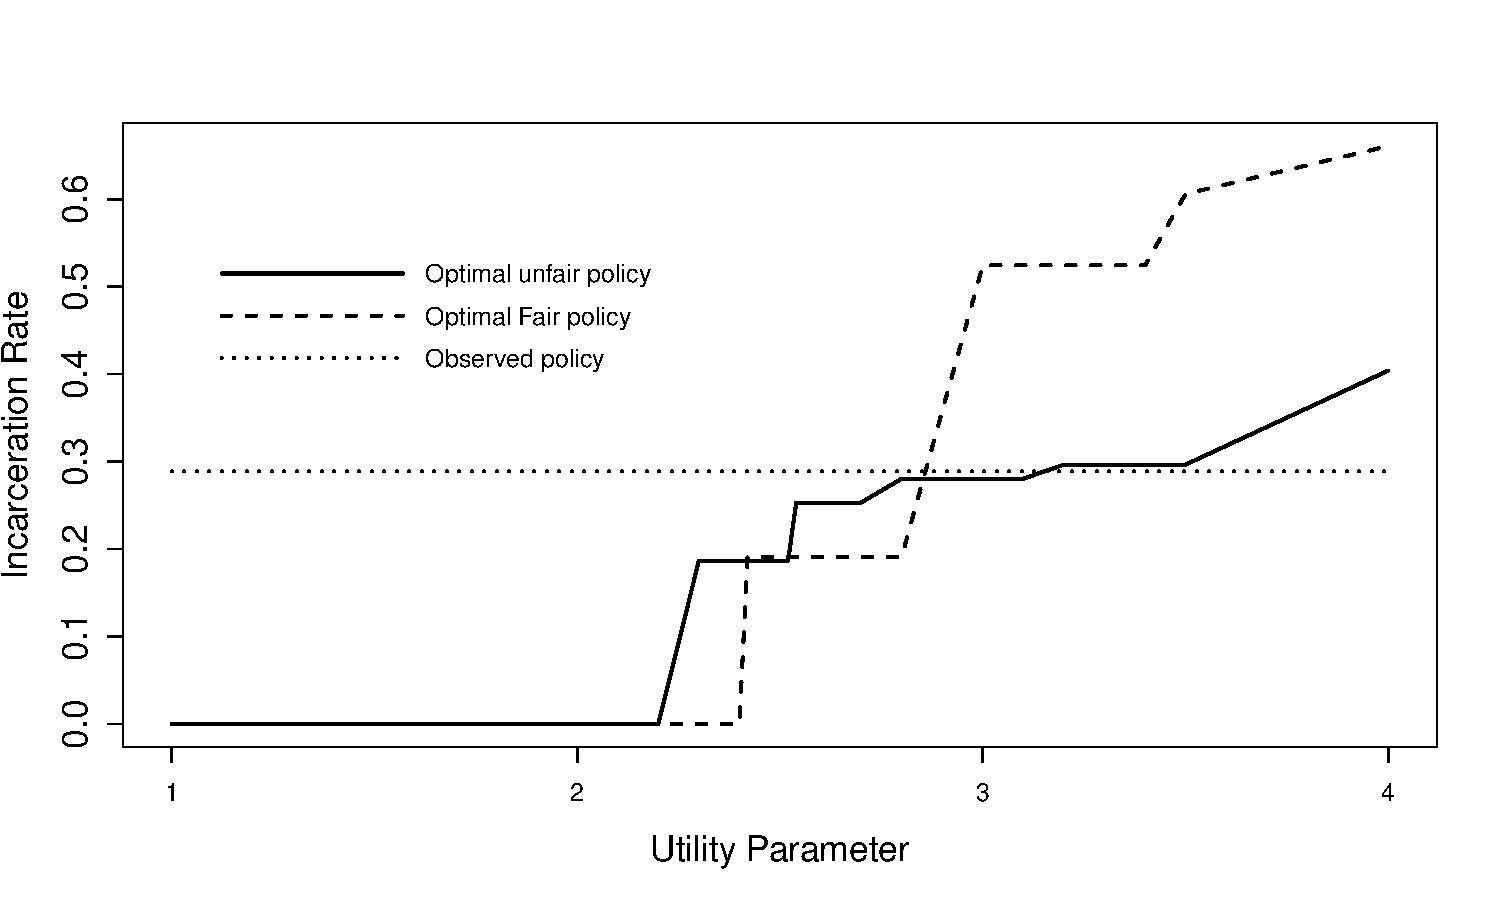
\includegraphics[scale=.32]{OverallRate.pdf}
	\end{center}
	\caption{Overall incarceration rates for the COMPAS data as a function of the utility parameter $\theta$.}
\end{figure}
\begin{figure}[t!] 
	\begin{center}
		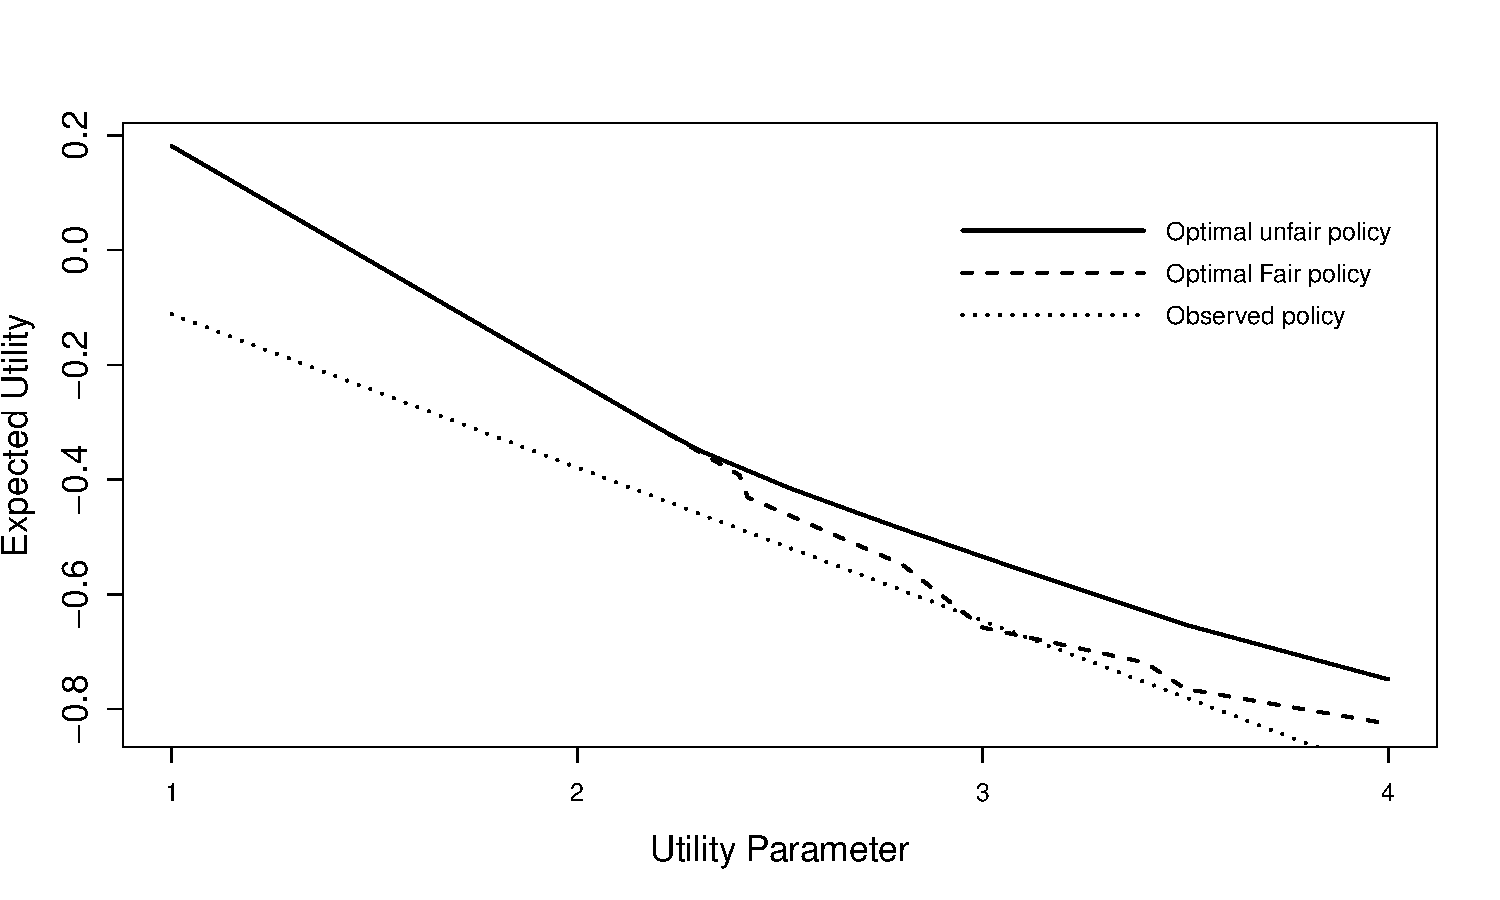
\includegraphics[scale=.32]{ExpectedUtility.pdf}
	\end{center}
	\caption{The relative utility of policies for the COMPAS data as a function of the utility parameter $\theta$.}
\end{figure}


\newpage
\section*{Appendix D: Proofs}

\begin{thm}%{\ref{thm:est}}
	Assume $S$ is binary. Under the causal model above, the following are consistent estimators of PSE$^{sy}$ and PSE$^{sa_k}$, assuming all models are correctly specified:
	{\small
		\begin{align}
			&\widehat{g}^{sy}(Z) = \\ \nonumber 
			&\frac{1}{N} \sum_{n=1}^{N} \Big\{ \frac{\mathbb{I}(S_n = s)}{p(S_n | X_n)} \ \frac{p(M_{n} | s', X_n)}{p(M_{n} | s, X_n)}
			- \frac{\mathbb{I}(S_n = s')}{p(S_n | X_n)} \Big\} \ Y_n \\ \nonumber \\
			%\label{eq:ipwSY}
			%		\end{align} 
			%	}
			%	{\small
			%		\begin{align}
			&\widehat{g}^{s{a}_k}(Z) =\\ \nonumber 
			&\frac{1}{N} \sum_{n=1}^{N} \Big\{ \frac{\mathbb{I}(S_n = s)}{p(S_n | X_n)} \ \frac{p(M_{n} | s', X_n)}{p(M_{n} | s, X_n)}
			- \frac{\mathbb{I}(S_n = s')}{p(S_n | X_n)} \Big\} \ A_{kn}
			%\label{eq:ipwSA}
		\end{align}
	}%
\end{thm}
\begin{prf}
	The latent projection \cite{verma90equiv} of any $K$ stage DAG onto $X,S,M,A,Y$ suffices to identify and estimate the two path-specific effects in question, and this latent projection is the complete DAG with topological ordering $X,S,M,A,Y$.
	The consistency of the estimators above then follows directly from derivations in \cite{tchetgen12semi}.
	As an example, we have the following derivation for the first term of $g^{sy}(Z)$:
{\small
	\begin{align*}
	&
	\sum_{X,M} \E\left[
	Y| s, M, X
	\right]p(M|s',X)p(X)\\
	&= \sum_{X,M,A,Y} Y p(Y | s,M,A,X) p(A | s,M,X) p(M | s',X) p(X)\\
	&=
	\sum_{X,S,M,A,Y} \frac{\mathbb{I}(S = s)p(M | s', X)}{p(S | X) p(M | s, X)} Y %\E[Y | s, M, A, X]
	dp(Y,S,M,A,X)\\
	%&=
	%\int \E[Y | s, M, A, X] p(A | s,M,X) p(M | s',X) p(X)\\
	&= \E\left[
	\frac{\mathbb{I}(S = s)p(M | s', X)}{p(S | X) p(M | s, X)} Y %\E[Y | s, M, A, X]
	\right]\\
	\end{align*}
}%
	which is precisely the identifying functional for the first term of the PSE we are interested in. That the above estimator is consistent for this functional is a standard result.
\end{prf}

\begin{thm}
	Consider the K-stage decision problem described by the DAG in Fig 1c. Let $p^*(M|S,X; \alpha_{m})$ and $p^*(S|X; \alpha_s)$ be the constrained models chosen to satisfy PSE$^{sy} = 0$ and PSE$^{sa_k} = 0$. Let $\tilde{p}(Z)$ be the joint distribution induced by $p^*(M|S,X; \alpha_{m})$ and $p^*(S|X;\alpha_s)$, and where all other distributions in the factorization are unrestricted. That is,
	{\small
		\begin{align*}
		\tilde{p}(Z) \equiv p(X)p^*(S|X;\alpha_s) &p^*(M|S,X;\alpha_m)\\
		&\times \prod_{k=1}^K p(A_k|H_k) p(Y_k|A_k,H_k).\\
		\end{align*}
	}%
	Then the functionals PSE$^{sy}$ and PSE$^{sa_k}$ taken w.r.t.\ $\tilde{p}(Z)$ are also zero.
\end{thm}
\begin{prf}
Let $Y \equiv Y_K$.  Because $M$ preceeds all $A_k,Y_k$ for $k = 1, \ldots K$, it suffices to consider the latent projection
with only variables $X,S,M,A,Y$ without affecting identifiability considerations.  Then we have the following:
{\small
	\begin{align*}
	&\widetilde{\text{PSE}}^{sy} \\
	&= \tilde{\E}[Y(s,M(s'))] - \tilde{\E}[Y(s')] \\ 
	&= \sum_{X,M} \{ \tilde{\E}[Y | s,M,X] - \tilde{\E}[Y | s',M,X] \} p^*(M | s',X;{\alpha}_m) p(X) \\
	&= \sum_{X,M} \{ {\E}[Y | s,M,X] - {\E}[Y | s',M,X] \} p^*(M | s',X;{\alpha}_m) p(X) \\
	&= \sum_{X,M,Y} Y \{ p(Y | s,M,X) - p(Y | s',M,X) \} p^*(M | s',X;{\alpha}_m) p(X) \\
	%		\end{align} 
	%	}
	%	{\small
	%		\begin{align}
	%&= \E \Big[ \Big\{ \frac{\mathbb{I}(S = s)}{p^*(S | X;\hat{\alpha}_s)} \ \frac{p^*(M | s', X;\hat{\alpha}_m)}{p^*(M | s, X;\hat{\alpha}_m)}
	%- \frac{\mathbb{I}(S = s')}{p^*(S | X;\hat{\alpha}_s)} \Big\} \ Y \Big] \\
	&= \sum_{X,S,M,Y} Y \Big\{ \frac{\mathbb{I}(S = s)}{p^*(S | X;\alpha_s)} \ \frac{p^*(M | s', X;\alpha_m)}{p^*(M | s, X;\alpha_m)}
	- \frac{\mathbb{I}(S = s')}{p^*(S | X;\alpha_s)} \Big\}  \\
	& \times p(Y | M,S,X) p^*(M | S,X; \alpha_m) p^*(S | X; \alpha_s) p(X)\\
	%&= \E \Big[ Y \Big\{ \frac{\mathbb{I}(S = s)}{p^*(S | X;\hat{\alpha}_s)} \ \frac{p^*(M | s', X;\hat{\alpha}_m)}{p^*(M | s, X;\hat{\alpha}_m)}
	%- \frac{\mathbb{I}(S = s')}{p^*(S | X;\hat{\alpha}_s)} \Big\} \Big] \\
	&=0
	%= \sum_{x,m} &\{ \tilde{\E}[\frac{\mathbb{I}(S=s)}{p^*(S|X;\hat{\alpha}_s)} \ \frac{p(M | s', X)}{p(M | s, X)} Y] - \tilde{\E}[Y | s',M,X] \} p^*(M | s',X;\hat{\alpha}_m) p(X)
	\end{align*}
}%
by choice of $p^*(M |S, X;\alpha_m)$ and $p^*(S | X;\alpha_s)$.
The proof is structurally the same for $\widetilde{\text{PSE}}^{sa_k}$.
\end{prf}

\section*{Appendix E: Modified results with multiple sets of mediators}
In the main paper, we discussed a $K$-stage decision problem with one set of permissible mediators, $M$. Here, we extend those results to the setting where we have multiple sets of mediators $M_1, \ldots, M_K$, i.e., a DAG with topological ordering $X, S, M_1, A_1, Y_1, \ldots, M_K, A_K, Y_K$. In this case, we consider the following paths impermissible: PSE$^{sy}$, representing the effect of $S$ on $Y$ along all paths \emph{other than} the paths of the form $S \to M_k \to \ldots \to Y$ ($\forall k$); and PSE$^{sa_k}$, representing the effect of $S$ on $A_k$ along all paths \emph{other than} the paths of the form $S \to M_j \to \ldots \to A_k$ ($\forall j \leq k$). That is, we consider \emph{only} pathways connecting $S$ and $A_k$ or $Y$ through the allowed mediators $M_1, \ldots, M_K$ to be fair. In this case, the PSEs are identified by a modification of the previous formula given in Section 3.2. 
%
{\small
\begin{align*}
	&\text{PSE}^{sy} = \E[Y(s,M_1(s'),\ldots,M_K(s'))] - \E[Y(s')] \\ 
	&= \sum_{x,\overline{m}_K,\overline{a}_{K-1},\overline{y}_{K-1},} \{ \E[Y | s,\overline{M}_K, \overline{A}_{K-1},\overline{Y}_{K-1},X]\\
	&- \E[Y | s', \overline{M}_K, \overline{A}_{K-1},\overline{Y}_{K-1},X] \} \prod_{k=1}^K p(M_k | s',\overline{A}_{k-1},\overline{Y}_{k-1},X)\\
	&\times \prod_{k=1}^{K-1} p(A_k | s, \overline{M}_k,\overline{A}_{k-1},\overline{Y}_{k},X) p(Y_k | s,\overline{M}_k,\overline{A}_{k},\overline{Y}_{k-1},X) p(X) 
	\\
	&\mbox{}
\end{align*}
}

\vspace{-1.5cm}
{\small
\begin{align*}
	&\text{PSE}^{sa_k} = \E[A_k(s,M_1(s'),\ldots,M_K(s'))] - \E[A_k(s')] \\ 
	&= \sum_{x,\overline{m}_k,\overline{a}_{k-1},\overline{y}_{k-1},} \{ \E[A_k | s,\overline{M}_k, \overline{A}_{k-1},\overline{Y}_{k-1},X]\\
	&- \E[A_k | s', \overline{M}_k, \overline{A}_{k-1},\overline{Y}_{k-1},X] \} \prod_{k=1}^K p(M_k | s',\overline{A}_{k-1},\overline{Y}_{k-1},X)\\
	&\times \prod_{j=1}^{k-1} p(A_j | s, \overline{M}_j,\overline{A}_{j-1},\overline{Y}_{j},X) p(Y_j | s,\overline{M}_j,\overline{A}_{j},\overline{Y}_{j-1},X) p(X)
\end{align*}
}%
With these definitions, we can replace the estimators in Theorem 1 with:
{\small
	\begin{align*}
	&\widehat{g}^{sy}(Z) = \\ \nonumber 
	&\frac{1}{N} \sum_{n=1}^{N} \Big\{ \frac{\mathbb{I}(S_n = s)}{p(S_n | X_n)} \ \prod_{k=1}^K \frac{p(M_{k,n} | s', \overline{A}_{k-1,n},\overline{Y}_{k-1,n}, X_n)}{p(M_{k,n} | s, \overline{A}_{k-1,n},\overline{Y}_{k-1,n}, X_n)}\\
	&- \frac{\mathbb{I}(S_n = s')}{p(S_n | X_n)} \Big\} \ Y_n 
	\\  \\
	&\widehat{g}^{sa_k}(Z) =\\ \nonumber 
	&\frac{1}{N} \sum_{n=1}^{N} \Big\{ \frac{\mathbb{I}(S_n = s)}{p(S_n | X_n)} \ \prod_{k=1}^K \frac{p(M_{k,n} | s', \overline{A}_{k-1,n},\overline{Y}_{k-1,n}, X_n)}{p(M_{k,n} | s, \overline{A}_{k-1,n},\overline{Y}_{k-1,n}, X_n)} \\
	&- \frac{\mathbb{I}(S_n = s')}{p(S_n | X_n)} \Big\} \ A_{kn} \nonumber
	%\label{eq:ipwSA}
	\end{align*}
}%
Then, in Theorem 2 we analogously define $\tilde{p}(Z)$ as follows:
{\small
	\begin{align*}
	\tilde{p}(Z) \equiv p(X)p^*(S|X;\alpha_s) \prod_{k=1}^K \Big\{ &p^*(M_k|S,\overline{A}_{k-1},\overline{Y}_{k-1},X;\alpha_{m})\\
	&\times p(A_k|H_k) p(Y_k|A_k,H_k) \Big\}.\\
	\end{align*}
}%
In this case we constrain the $S$ and $M_k$ models $\forall k$, the rest of the procedure remaining the same.
Aside from the form of the identifying functional, the proofs of modified versions of Theorem 1 and Theorem 2 are analogous.

{\small
	\bibliographystyle{plainnat}
	%\bibliographystyle{plain}
	\bibliography{references}
}
\end{document}
